\chapter{套筒}
\begin{figure}[htbp]
\centering
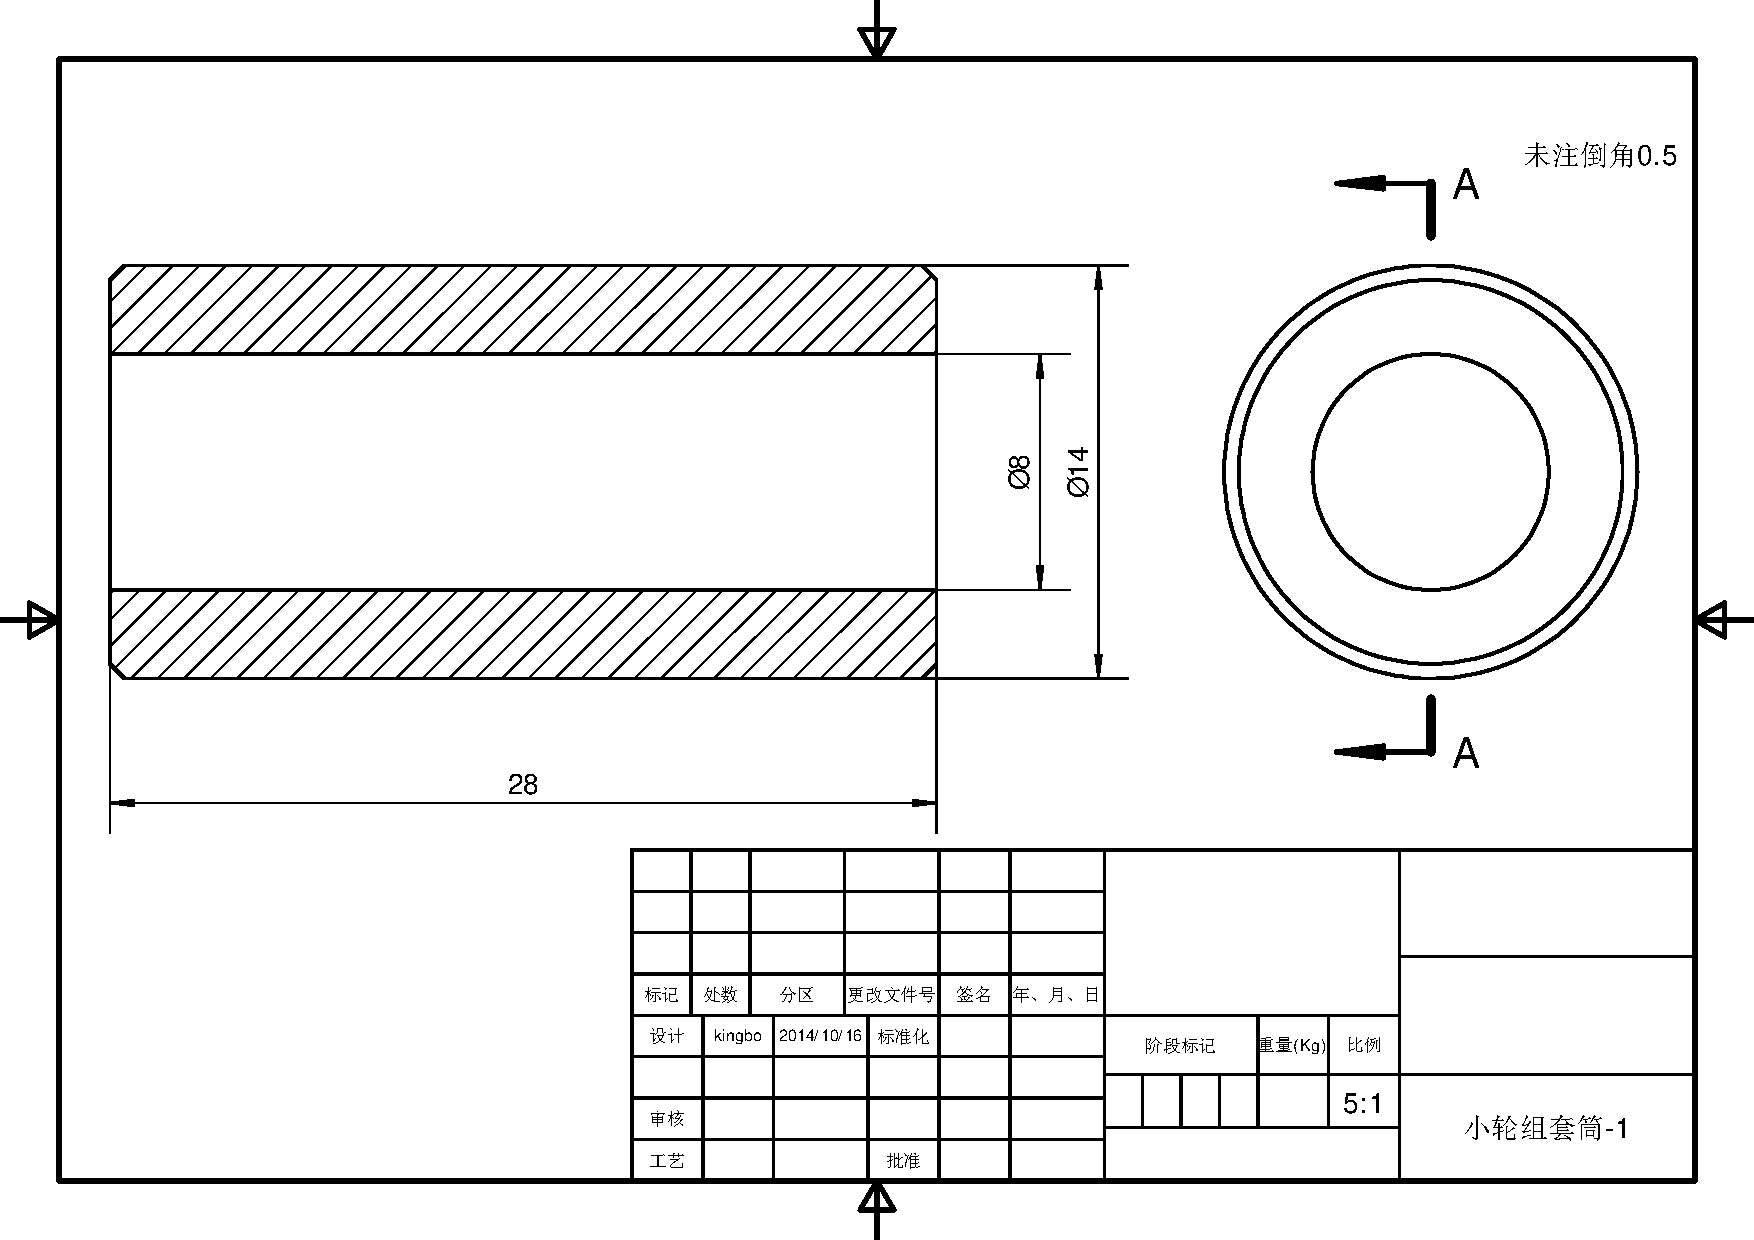
\includegraphics[scale=0.45]{xiaoluntaotong.pdf}
\caption{套筒零件图}\label{fig:xiaoluntaotong}
\end{figure}
%AutoCAD作为国际上广泛使用的流行的绘图工具,它具有较强的二维绘图和三维绘图功能,欢迎来到AutoCAD的三维世界,
本章我们的目标是用AutoCAD制作图\ref{fig:xiaoluntaotong}所示的小轮组构成零件轮轴的三维模型,并以此展开我们的AutoCAD三维建模之旅。本章将讲述以下内容:
\begin{itemize}
	\item 零件图的组成
	\item 圆柱体的构建
	\item 差集操作
	\item 倒角操作
	\item 视图的切换
	\item 三视图的形成
\end{itemize}
\section{初识零件图}
在构建图\ref{fig:xiaoluntaotong}所示零件之前,让我们先来了解一些相关的制图知识。类似于图\ref{fig:xiaoluntaotong}所示的图纸被称为零件图。所谓零件图是用于表达零件的图样,它广泛运用于工程技术设计、施工或产品制造,它是制造、加工、测量、检验的依据,是工程界的共同技术语言,是表达和交流技术思想的必备工具,是工程技术部门的一项重要技术文件。掌握零件图的阅读和绘制不仅是构建零件三维模型的基础,也是从事工程设计和技术的工程技术人员所必须具备的基本能力。一张完整的零件图应包括以下几个组成部分:
\begin{itemize}
\item 一组视图
根据国家制图标准规定的视图、剖视、剖面及其他画法绘制的用于表达零件内外形状的图形。
\item 完整的尺寸
用于确定零件各部分形状大小和位置的全部尺寸。它是按照国家标准GT/T4458.4-1984的要求进行标注的。
\item 技术要求
用于规定零件在制造和检验时应达到的一些要求。通常用规定的符号标注于图纸中或在图纸上指定位置用文字统一标出。
\item 标题栏
用于说明零件的名称、材料、数量等信息。它是按照国家标准GB/T10609.1-1989的规定绘制的。
\end{itemize}
\begin{figure}[htbp]
\centering
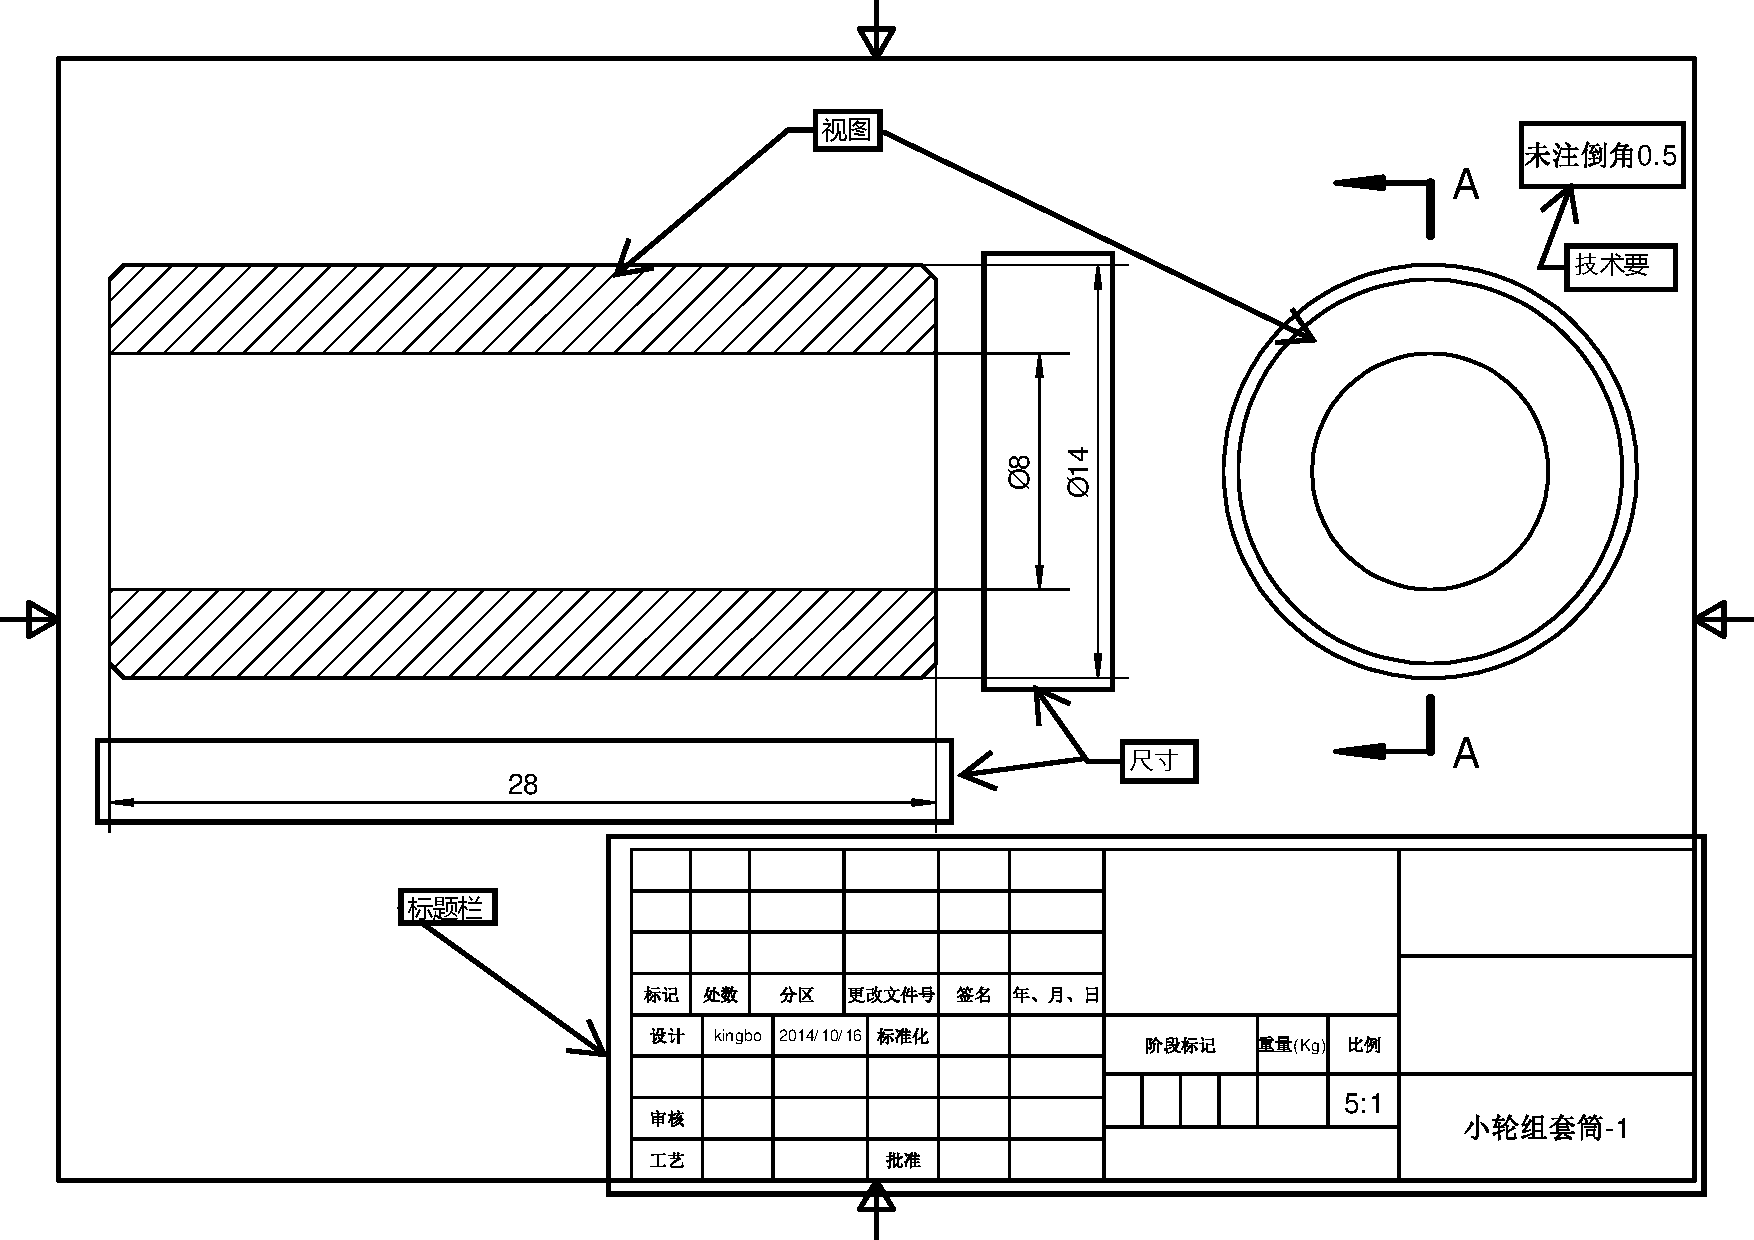
\includegraphics[scale=0.45]{xiaoluntaotong2.pdf}
\caption{零件图组成部分}\label{fig:xiaoluntaotong2}
\end{figure}
图\ref{fig:xiaoluntaotong2}对图\ref{fig:xiaoluntaotong}所示零件图的各个组成部分进行了标注。
\section{圆柱体视图}
图\ref{fig:xiaoluntaotong}所示零件图中的视图既然是用于表达零件的内外形状的,那么它的立体形状是怎样的呢,如保用AutoCAD构建出它的三维模型呢?要解决这个问题,我们先将图\ref{fig:xiaoluntaotong}所示零件图进行简化,忽略其内部及细微的局部,只研究其中$\phi 14$所对应的部分,简化后的结果如图\ref{fig:yuanzhuti}所示。
\begin{figure}[htbp]
\centering
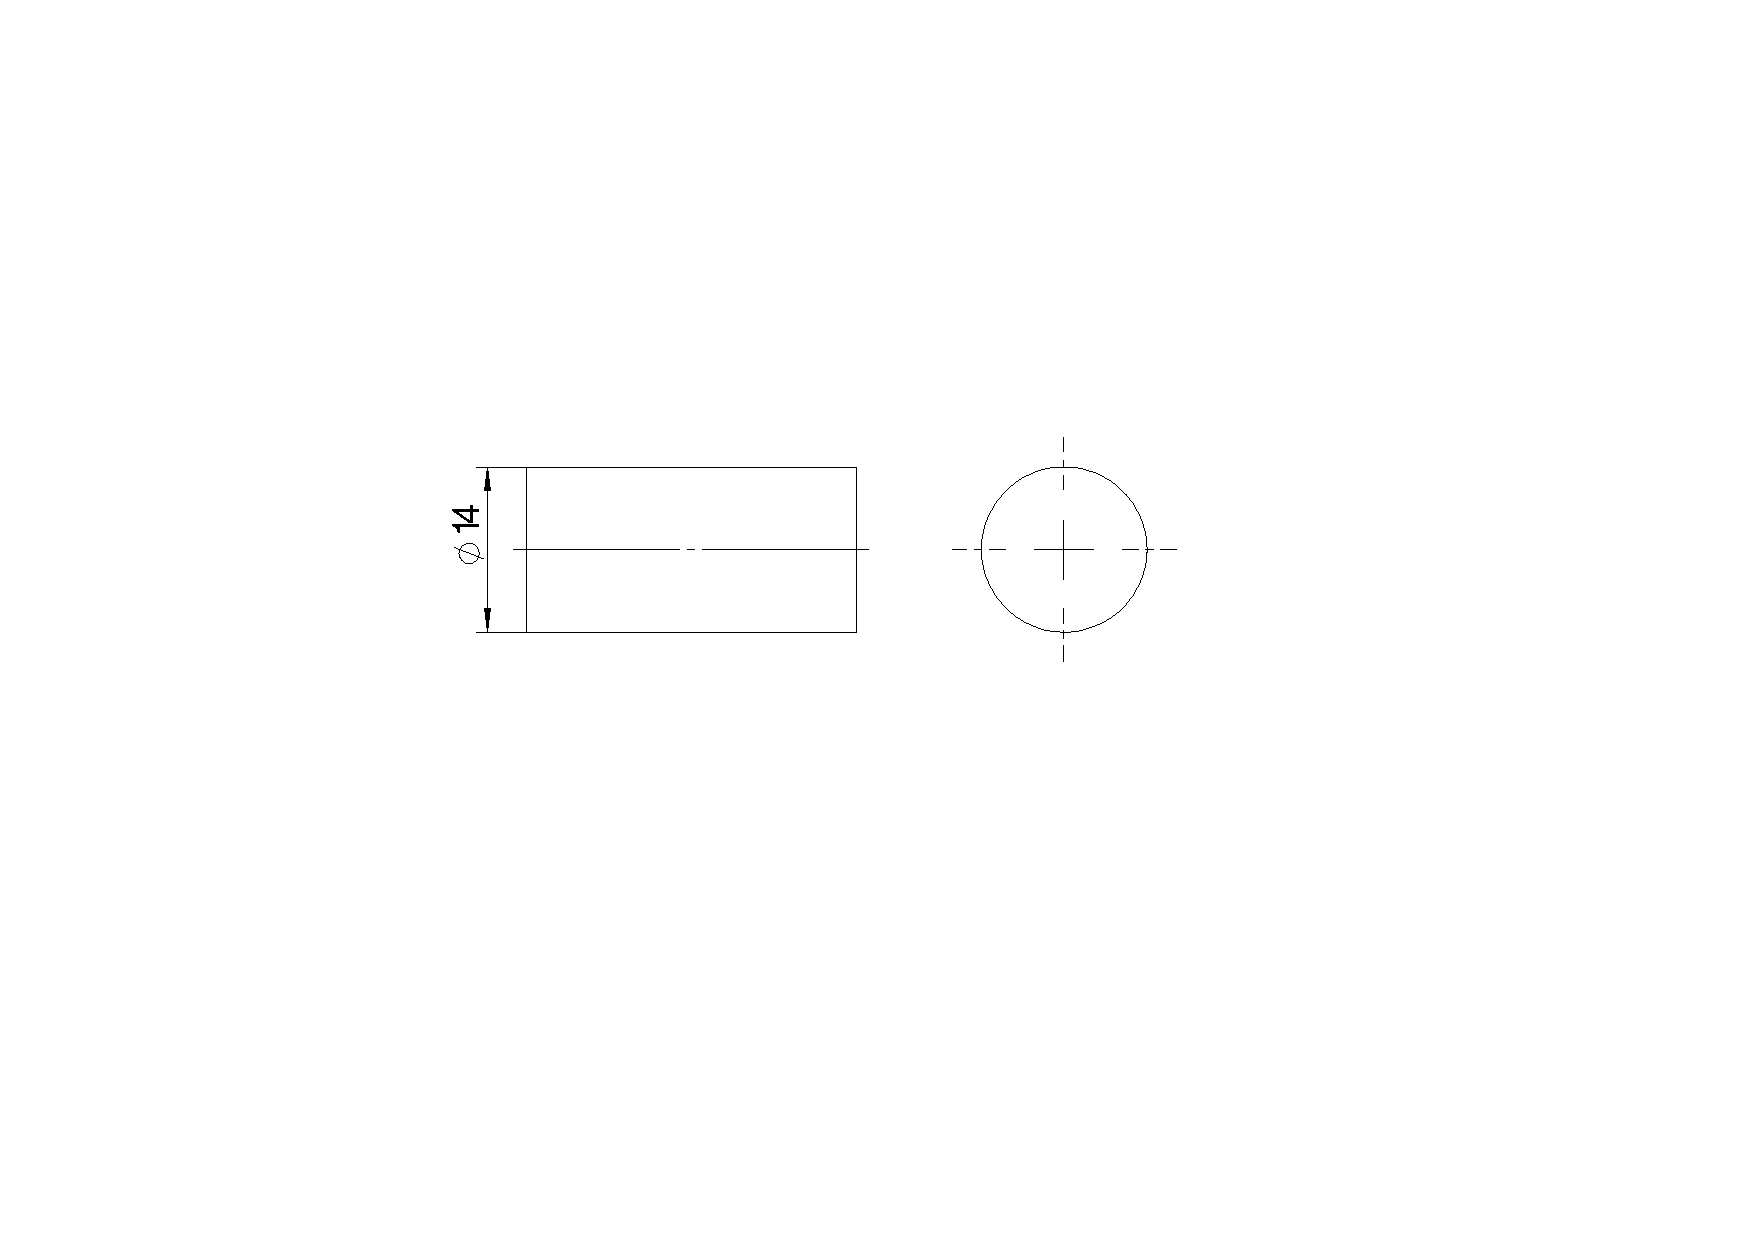
\includegraphics[scale=0.55]{yuanzhuti.pdf}
\caption{套筒外圆柱视图}\label{fig:yuanzhuti}
\end{figure}

那么图\ref{fig:yuanzhuti}所表达的又是什么物体呢?要回答这个问题,我们先将一个圆柱体放置于图\ref{fig:sanweizuobiao}所示的三个相互垂直的三面投影之中,然后从三个方向将圆柱体投影到投影面上,即可得到圆柱体的三面投影,如图\ref{fig:yuanzhutouyin}所示。从圆柱体的三面投影可以看出其中两投影的大小和形状是一样的,均为矩形,仅有一个投影为圆。
\begin{figure}[htbp]
\centering
\subfloat[三维投影面]{\label{fig:sanweizuobiao}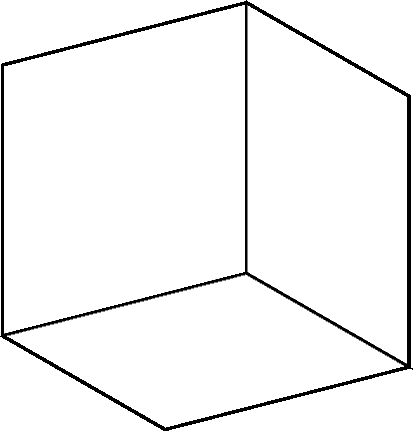
\includegraphics[scale=0.4]{sanweizuobiao.png}}\hspace{30pt}
\subfloat[圆柱体三面投影]{\label{fig:yuanzhutouyin}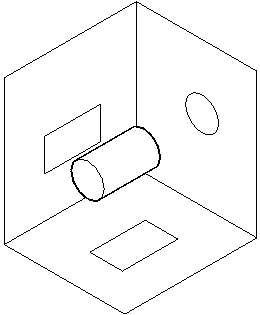
\includegraphics[scale=0.3]{yuanzhutouyin.png}}
\end{figure}

由此可以看出图\ref{fig:yuanzhuti}所示的视图表达的是一个直径为$\phi 14$,长为28的圆柱体,其中符号$\phi$用于表示后面所标注的尺寸是直径。

\endinput
\section{套筒三维模型构建}\label{sec:taotongjianmo}
基于上面的认识和理解,现在可以用AutoCAD来构建套筒的三维模型,具体构建方法是:
\begin{procedure}

\item 启动AutoCAD软件。

启动AutoCAD软件的方法通常有:
\begin{itemize}
\item 双击桌面图标
\includegraphics[scale=0.2]{cadicon.png}。
\item 【开始】$\rightarrow$ 【所有程序】$\rightarrow$【Autodesk】$\rightarrow$【AutoCAD 2014 – 简体中文 (Simplified Chinese)】$\rightarrow$【AutoCAD 2014 – 简体中文 (Simplified Chinese)】。
\end{itemize}
AutoCAD软件启动完成后,将出现图\ref{fig:cadui}所示的软件界面。
\begin{figure}[htbp]
\centering
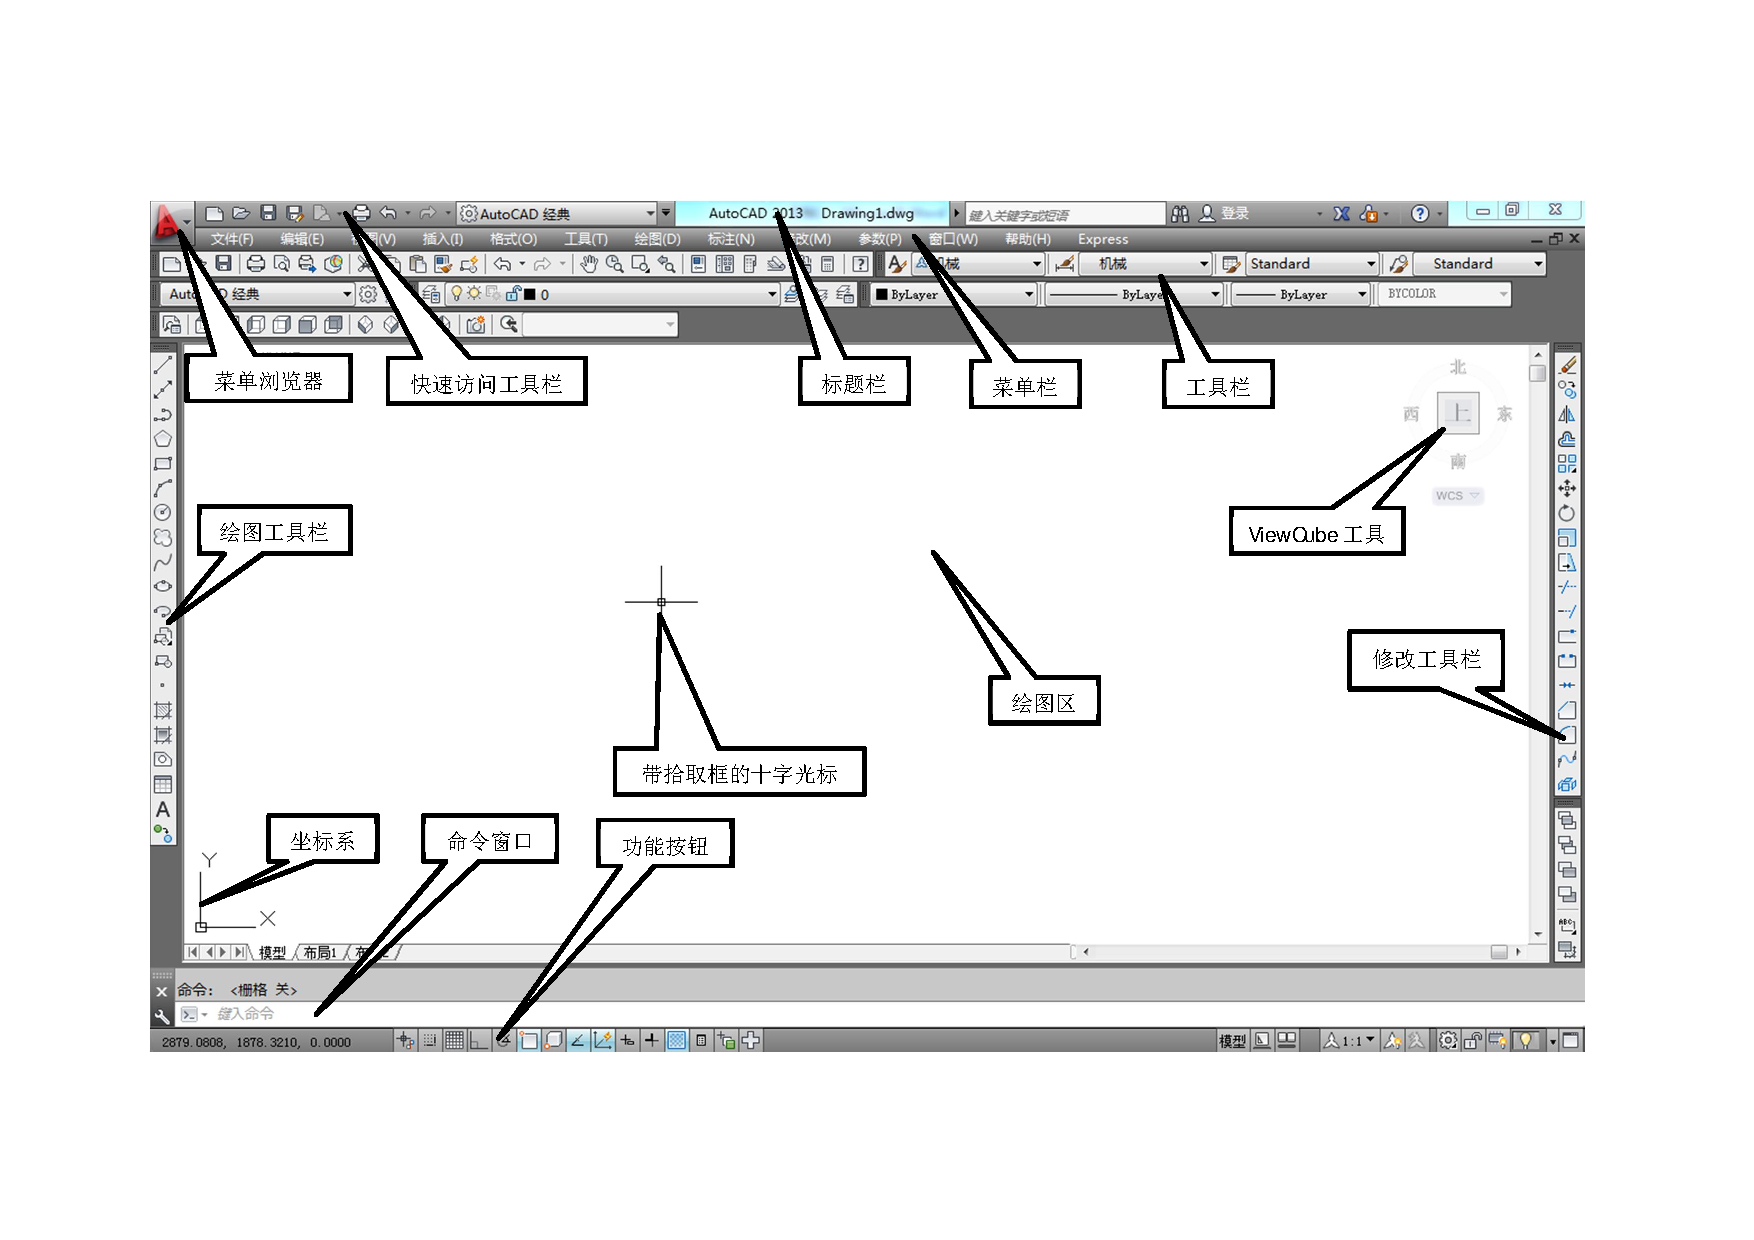
\includegraphics[scale=0.5]{cadui.pdf}
\caption{“AutoCAD经典”工作空间}\label{fig:cadui}
\end{figure}
AutoCAD软件的界面与Word字处理软件的界面非常相似,也是由标题栏、菜单栏、工具栏、绘图区、状态栏等要素构成。不同的是AutoCAD软件的界面在标题栏上还有菜单浏览器和快速访问工具栏;绘图区的左下方有坐标系,右上方有ViewCube工具,左边有绘图工具栏,右边有编辑工具栏;状态栏的上方有命令窗口;状态栏中有功能按钮。

\item 将视图切换为左视图。

AutoCAD启动后默认的视图方向是俯视图方向,而套筒零件的特征图位于左视图方向,为使套筒零件的三维模型与纸方向一致,需要将AutoCAD的视图方向切换为左视图方向。实现左视图切换的方法有:
\begin{itemize}
\item 键盘输入-VIME\index{-view,视图} 或-V,选择【正交】选项中的【左视】项。
\item 键盘输入-VIME,并输入left。
\item 【视图】$\rightarrow$【三维视图】$\rightarrow$【左视图】。
\item 【视图】$\triangleright$【左视】图标
\includegraphics[scale=0.6]{lefttool.png}。
\end{itemize}
同理,如果要将视图切换为其它视图方向,其操作方法与切换左视图的方法是一致的,只是需要将“左视”换成其它视图方向即可。例如要将视图方向切换为俯视图方向则将上述方法中的【左视】改为【俯视】。

\begin{lstlisting}
命令: -VIEW
输入选项 [?/删除(D)/正交(O)/恢复(R)/保存(S)/设置(E)/窗口(W)]: left
\end{lstlisting}

\yaodian{结合能够显著表达物体特征的视图选择AutoCAD的三维视图方向,将有助于三维模型的构建。}

\item 构建外圆柱
在AutoCAD中,创建圆柱体需要用到圆柱体命令,通常启动【圆柱体】命令的方法有:
\begin{itemize}
\item 键盘输入CYLINDER\index{cylinder,圆柱体}或CYL。
\item 【绘图】$\rightarrow$【建模】$\rightarrow$【圆柱体】。
\item 【建模】$\triangleright$【圆柱体】图标
\includegraphics[scale=0.6]{cylinder.png}。
\end{itemize}
在图\ref{fig:commandline}所示的命令行窗口中输入CYLINDER命令,并回车或按空格键结束命令。结束命令输入后,绘图区中的光标形状由带拾取框的十字光标“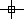
\includegraphics[scale=0.8]{guangbiao1} ”变成十字形光标“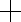
\includegraphics[scale=0.6]{guangbiao2}”,表示此时AutoCAD进入了绘图状态。
\begin{figure}[htbp]
\centering
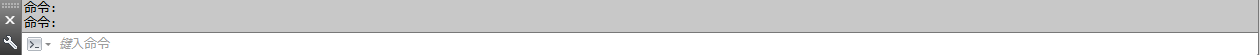
\includegraphics[scale=0.35]{commandline.png}
\caption{AutoCAD命令行}\label{fig:commandline}
\end{figure}

\yaodian{AutoCAD命令行是重要的信息窗口,是正确绘图的关键。初学者应多关注命令行的提示。}
\begin{lstlisting}
命令: _CYLINDER
\end{lstlisting}
接下来命令提示行中会提示,指定圆柱体的底面中心点或者绘图选项。
\begin{lstlisting}
指定底面的中心点或 [三点(3P)/两点(2P)/切点、切点、半径(T)/椭圆(E)]:
\end{lstlisting}
看到上述提示后,可以用鼠标在绘图区中任意单击一下,以完成底面中心点的指定,也可能输入其它选项来指定底面。

接下来,命令提示输入底面的半径,此时根据$\phi 14$直径尺寸计算得到半径应该是7,因此直接从键盘上输入数字7并按空格键或回车键结束半径的指定。如果要指定直径则需要在指定半径的提示下,输入选项字母D来进入指定直径状态。
\begin{lstlisting}
指定底面半径或 [直径(D)]: 7
\end{lstlisting}
最后,命令提示指定圆柱体的高度,此时从键盘上输入数字28,并按回车或空格键结束高度指定。
\begin{lstlisting}
指定高度或 [两点(2P)/轴端点(A)]: 28
\end{lstlisting}
此时,绘图区的光标切换为带拾取框的十字光标,表示AutoCAD当前处于非绘图命令状态。
\item 将视图方向切换为西南等轴测。
\begin{lstlisting}
命令: -VIEW
-VIEW输入选项 [?/删除(D)/正交(O)/恢复(R)/保存(S)/设置(E)/窗口(W)]:  swiso
\end{lstlisting}
完成视图切换后,可以看到图\ref{fig:taotong1} 所示的结果。
\begin{figure}[htbp]
\centering
\subfloat[]{\label{fig:taotong1}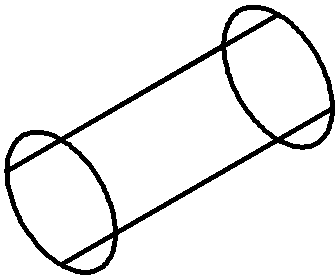
\includegraphics[scale=0.3]{taotong1.png}}\hspace{20pt}
\subfloat[]{\label{fig:centerselect}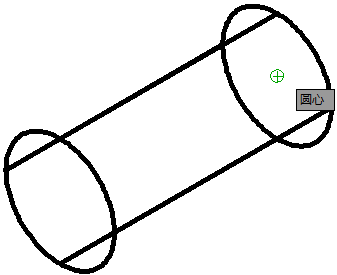
\includegraphics[scale=0.3]{centerselect.png}}\hspace{20pt}
\subfloat[]{\label{fig:taotong2}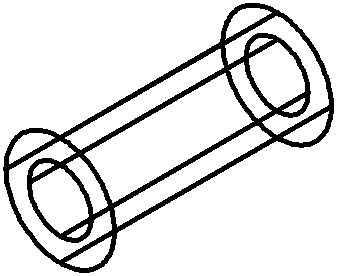
\includegraphics[scale=0.3]{taotong2.png}}
\caption{构建圆柱体}
\end{figure}

\item 构建内圆柱
\begin{lstlisting}
命令: _CYLINDER
指定底面的中心点或 [三点(3P)/两点(2P)/切点、切点、半径(T)/椭圆(E)]:
\end{lstlisting}
当命令提示指定底面圆心时,为保证我们所绘制的$\phi 8$圆柱与$\phi 14$圆上下端面对齐并且同轴,需要应用AutoCAD的对象后捕捉方式来选取$\phi 14$圆底端面的圆心作为$\phi 8$圆柱底端面的圆心。其具体操作方法是:将鼠标移至图\ref{fig:centerselect}所示的位置,直到出现图示的圆心标记和提示,然后单击鼠标左键确定圆柱体的圆心,并按下面的提示完$\phi 8$圆柱体的构建。
\begin{lstlisting}
指定底面半径或 [直径(D)] <7.0000>: 4
指定高度或 [两点(2P)/轴端点(A)] <28.0000>:
\end{lstlisting}

\yaodian{合理使用捕捉是实现精确绘图和快速绘图的重要方法之一。}

\item 进行差集操作,制作内孔

由于前面构建的是两个实体的圆柱体,因此并没有真构成套筒零件所需要的孔,而实现孔的构建则需要从$\phi 14$的圆柱体中去除一个$\phi 8$的圆柱体,要实现这一目标,需要用到实体编辑中的【差集】命令,其启动方法有:
\begin{itemize}
\item 键盘输入SUBTRACT\index{subtract,差集}或SU。
\item 【修改】$\rightarrow$【实体编辑】$\rightarrow$【差集】。
\item 【实体编辑】$\triangleright$【差集】图标
\includegraphics[scale=0.7]{subtracttool.png}。
\end{itemize}
\begin{figure}[htbp]
\centering
\subfloat[]{\label{fig:subtractselect}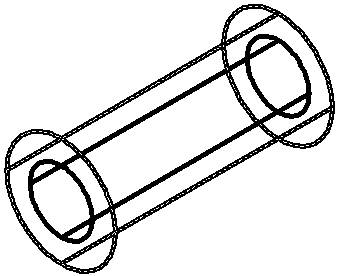
\includegraphics[scale=0.3]{subtractselect.png}}\hspace{40pt}
\subfloat[]{\label{fig:subtractselect1}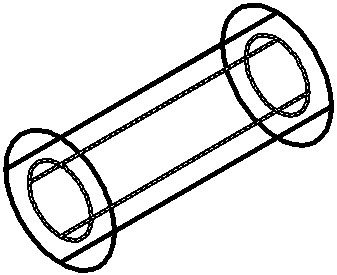
\includegraphics[scale=0.3]{subtractselect1.png}}
\caption{差集操作}
\end{figure}
\begin{lstlisting}
命令: SUBTRACT
选择要从中减去的实体、曲面和面域...
\end{lstlisting}
输入SUBTACT命令后,提示选择要从中减去的实体,同时绘图区的鼠标形状变为矩形小方框“
\includegraphics[scale=0.8]{selectobject.png}”,表示进入选择对象状态,此时按照图\ref{fig:subtractselect}所示选择$\phi 14$的圆柱体作为要从中减去的对象,并按回车或空格键结束选择。
\begin{lstlisting}
选择对象: 找到 1 个
选择对象:  选择要减去的实体、曲面和面域...
\end{lstlisting}
结束从中减去实体选择后,命令提示选择要减去的实体,此时按照图\ref{fig:subtractselect1}所示选择$\phi 8$圆柱体作为要选择的实体,并按驾车可空格键结束选择。
\begin{lstlisting}
选择对象: 找到 1 个
选择对象:
\end{lstlisting}
\item 进行倒角操作
至此,已经完成了套筒的整体部分的构建,还剩下两个倒角没有完成,在AutoCAD中完成三维立体倒角边构建的命令是“倒角边”,其启动方法有:
\begin{itemize}
\item 键盘输入CHAMFEREDGE\index{charmferedge,倒角边}。
\item 【修改】$\rightarrow$【实体编辑】$\rightarrow$【倒角边】。
\item 【实体编辑】$\triangleright$【倒角边】图标
\includegraphics[scale=0.6]{chamferedge.png}。
\end{itemize}

\begin{lstlisting}
命令: CHAMFEREDGE
距离 1 = 1.0000,距离 2 = 1.0000
\end{lstlisting}
启动完倒角边命令后,命令会提示当前的倒角边距离的默认值,并提示选择要倒角的边,此时按照图\ref{fig:chamferedgeselect}所示选择要倒角的一条边,选择完成后会自动生成倒角预览。
\begin{figure}[htbp]
\centering
\subfloat[]{\label{fig:chamferedgeselect}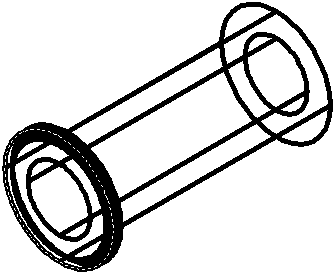
\includegraphics[scale=0.3]{chamferedgeselect.png}}\hspace{20pt}
\subfloat[]{\label{fig:chamferedgeselect1}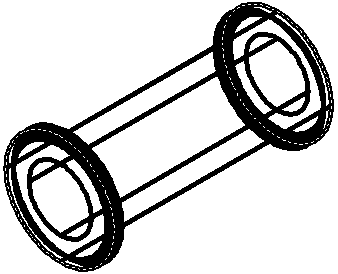
\includegraphics[scale=0.3]{chamferedgeselect1.png}}
\hspace{20pt}
\subfloat[]{\label{fig:chamferedgeresult}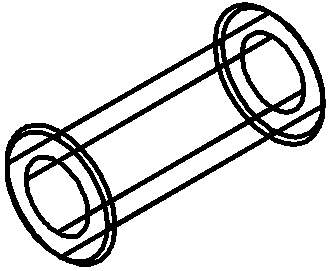
\includegraphics[scale=0.3]{chamferedgeresult.png}}
\caption{倒角边操作}
\end{figure}
\begin{lstlisting}
选择一条边或 [环(L)/距离(D)]:
\end{lstlisting}
接下来,按照图\ref{fig:chamferedgeselect1}所示,选择另一条要倒角的边。
\begin{lstlisting}
选择同一个面上的其他边或 [环(L)/距离(D)]:
\end{lstlisting}
套筒零件只有两个倒角边,因此选择倒角边至此结束,但是系统默认值并不是需要的倒距离,故需要选择距离(d)进行修改。
\begin{lstlisting}
选择同一个面上的其他边或 [环(L)/距离(D)]:d
\end{lstlisting}
最后将两个倒角距离均设置成为0.5,并用回车键接受,其结果如图\ref{fig:chamferedgeresult}所示。
\begin{lstlisting}
指定基面倒角距离或 [表达式(E)] <1.0000>: 0.5
指定其他曲面倒角距离或 [表达式(E)] <1.0000>: 0.5
按 Enter 键接受倒角或 [距离(D)]:
\end{lstlisting}
\item 进行着色
\begin{figure}[htbp]
\centering
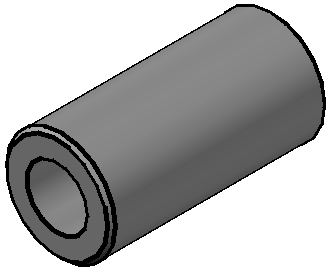
\includegraphics[scale=0.6]{taotonglititu.png}
\caption{套筒三维模型}\label{fig:taotonglititu}
\end{figure}
最后,将完成套筒三维模型以灰度方式的视觉样式进行着色,以使得三维模型看起更加真实。启动灰度视觉样式的方法有:
\begin{itemize}
\item 键盘输入 VSCURRENT\index{vscurrent,视觉样式}或VS,并输入G选项。
\item 【视图】$\rightarrow$【视觉样式】$\rightarrow$【灰度】。
\end{itemize}
\begin{lstlisting}
命令: vscurrent
输入选项 [二维线框(2)/线框(W)/隐藏(H)/真实(R)/概念(C)/着色(S)/带边缘着色(E)/灰度(G)/勾画(SK)/X 射线(X)/其他(O)] <二维线框>: G
\end{lstlisting}
完成灰度视觉样式切换后,其结果如图\ref{fig:taotonglititu}所示。

\item 保存模型

将建立好的套筒三维模型保存为“小轮组套筒.dwg”,AutoCAD中保存文件的方法有:
\begin{itemize}
\item 键盘输入SAVE\index{save,保存}或SAVEAS\index{saveas,另存为}。
\item 键盘输入\fbox{Ctrl}+\fbox{S}。
\item 【文件】$\rightarrow$【保存】或【另存为】。
\item 【工具栏】$\triangleright$【保存】图标
\includegraphics[scale=0.6]{savetool.png}。
\end{itemize}
调用保存命令后,会弹出图\ref{fig:saveasdialog}所示的文件保存对话框,此时在文件名处输入“小轮组套筒.dwg”,并单击保存。
\begin{figure}[htbp]
\centering
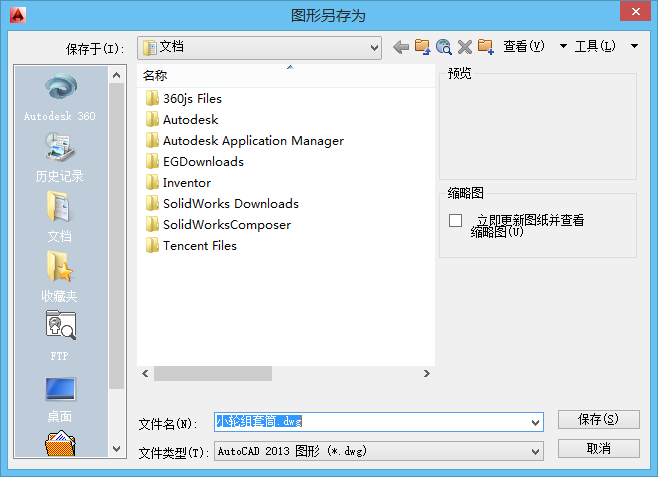
\includegraphics[scale=0.6]{saveasdialog.png}
\caption{保存文件对话框}\label{fig:saveasdialog}
\end{figure}
\end{procedure}

\endinput
\section{理解视图}
为什么图\ref{fig:xiaoluntaotong}所示的零件图能够唯一也表达\ref{fig:taotonglititu}所示的套筒零件呢,为什么需要两视图呢,一个视图能不能够表达呢,要回答这个问题,需要进一步了解一些与视图相关的知识。
\subsection{视图的概念}
\begin{figure}[htbp]
\centering
\subfloat[斜投影法]{\label{fig:xietouyinfa}
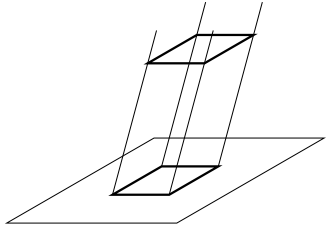
\includegraphics[scale=0.4]{xietoying.png}
}\hspace{30pt}
\subfloat[正投影法]{\label{fig:zhentouyinfa}
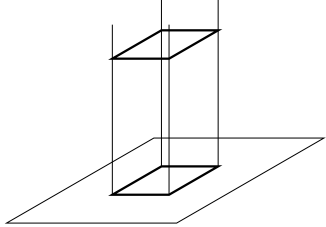
\includegraphics[scale=0.4]{zhengtouying.png}
}
\caption{平行投影法}\label{pingxingtouyin}
\end{figure}

 在图\ref{fig:xiaoluntaotong}所示的套筒零件图中,位于左边的图形称之为主视图,其表达式为全剖视图,关于全剖视图的概念及画法将在后面予以介绍。主视图清晰的表达了套筒零件的长度及内外结构。而位于右边的视图称之为左视图,它清楚地显示套筒零件为回转体类零件。

要理解什么是视图,首先需要了解投影的概念。投影是物体在阳光或灯光下所产生的影子。由于影子只能够表现物体轮廓而不能够表现物体的内部结果,工程实际中将物体内外空间几何元素加以抽象,并用不同的线型进行表示,实现物体内外细节的表达,从而形成的比较完备的、实用的投影方法。投影法分为中心投影法和平行投影法两类。所有投影线都互不平行且汇聚于点的投影法称为中心投影法。中心投影法主要用于绘制效果比较逼真的建筑或产品立体图。图\ref{pingxingtouyin}所示的投影法是平行投影法,从中可以看出其所有的投影线都是相互平行的,其中投影线倾斜于投影面则为斜投影,投影线垂直于投影面则为正投影法。工程中将用正投影法绘制的物体图形称为视图。
\begin{figure}[htbp]
\centering
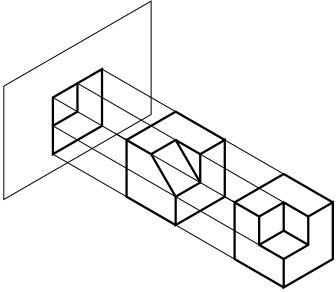
\includegraphics[scale=0.4]{buweiyi.png}
\caption{一个投影面不能确定物体在空间中的形状和位置}\label{fig:singleprojection}
\end{figure}
\subsection{三视图的形成}

\begin{figure}[htbp]
\centering
\subfloat[物体在三面投影中的投影]{\label{fig:threeviewprojection}
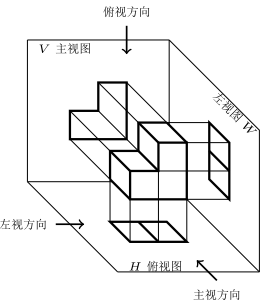
\includegraphics[scale=0.4]{wutisanmiantouying.png}}
\hspace{30pt}
\subfloat[三个投影面的展开]{\label{fig:threeviewzhankai}
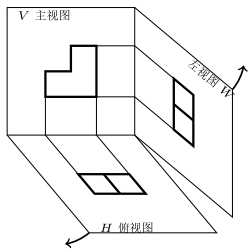
\includegraphics[scale=0.45]{touyingzhankai.png}}


\subfloat[展开后的三视图]{\label{fig:threeview}
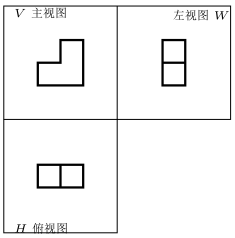
\includegraphics[scale=0.45]{zhankairesult.png}}
\hspace{30pt}
\subfloat[最终三视图]{\label{fig:threeviewguilu}
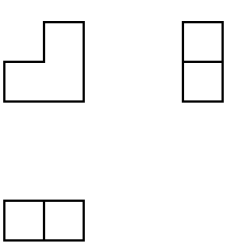
\includegraphics[scale=0.45]{sanshituresult.png}}
\caption{三视图的形成}
\end{figure}
了解完视图的概念后,让们来探讨一个视图能不能够准确地表达出物体的形状这个问题,首先让我们来看一下图\ref{fig:singleprojection}所示的投影。从图\ref{fig:singleprojection}中,我们可以看出不同的形状的物体在同一个视图投影面内具有相同的视图表示。之所以如此,主要是因为仅用一个视图只能反映物体两方向的尺寸,而空间物体需要用长宽高三个方向的尺寸帮能够将其大小形状完整清晰地表达出来。在没有尺寸标注的辅助的情况下,要解决投影只能够表达物体两个尺寸方向的问题,我们需要将物体向多个投影面进行投影,通过多个投影视图来实现物体上下、左右、前后各部分的形状和大小完整表达。在工程零件图中,通常都会使用两个或三个视图来表达一个零件。当然对于简单的轴类零件也经常使用一个视图来表达,对于特别复杂的零件还需要使用更多的辅助视图加以表达。但无论使用多少个视图,三视图是基本的零件图表达方式。下面,我们就来了解一下三视图的形成过程。




为此,我们需要根据国家标准规定,选三个相互垂直的投影面构成图\ref{fig:threeviewprojection}所示的三投影面体系。在三视图投影体系中,正对观察者的投影面称为正平面,用$V$表示。水平放置的投影面称水平面,用$H$表示。侧立的投影面称为侧平面,用$W$表示。将物体放置于三视图投影体系中,将其由前向后投影所得的$V$面视图称为主视;将其由上向下投影所得的$H$面视图称为府视图;将物体由左向右投影所得的$W$面视图称为左视图。最后,按照国家标准,以图\ref{fig:threeviewzhankai}所示方式展开,即以$V$面视图为基准,$H$面绕$V$面与$H$面的交线所形成的$X$轴向下旋转$90^o$;$W$面绕$V$面与$W$面的交线所形成的$Z$轴向右旋转$90^o$,使$V$、$H$、$W$面处于同一个平面内,如图\ref{fig:threeview}所示。展开后的三视图既不需要画边框和投影轴,也不需要标视图名称,如图\ref{fig:threeviewguilu}所示。

\subsection{三视图投影规律}
既然表达一个零件需要多个视图,那么这些视图之间就需要遵循一定规律,才能够准确的表示物体各个组成部分之间的关系。而视图之间所遵循的规律则称之为对应关系。图\ref{fig:threeviewguanxi}标识了三个视图之间的对应关系和视图所能表达的方位。从图中,我们可以得出:主视图反映物体的上下和左右关系,即反映物体的长和高;俯视图反映物体的左右和前后关系,即反映物体的长和宽;左视图反映物体的上下和前后,即反映物体的高和宽。因此,三视图的投影规律为:
\begin{itemize}
\item 主、俯视图长对正;
\item 主、左视图高平齐;
\item 俯、左视图宽相等。
\end{itemize}
\begin{figure}[htbp]
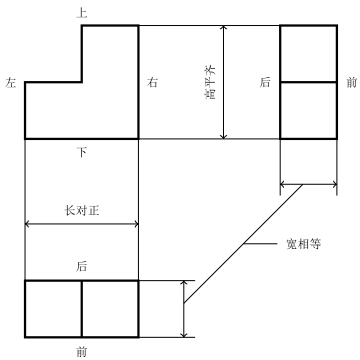
\includegraphics[scale=0.6]{touyingguilu.png}
\caption{三视图投影规律}\label{fig:threeviewguanxi}
\end{figure}
三视图的投影规律不仅适用于物体整体之间的投影,也适用于空间中的点、线面。同时它也是画图和读图的基础规则。由此可知,图\ref{fig:xiaoluntaotong}所示的套筒零件图中,主视图中$\phi 14$尺寸所标法的图线与左视图中的大圆处于同一条水平线上,符合高平齐的对应关系,表达了套筒的外形整体为圆柱体,与此类似,$\phi 8$则表达了套筒的内孔,紧邻大圆的中间圆则表达了倒角。

\endinput
\section{检验结果}
在了解了相关的视图知识后,让我们来简单地检验下套筒零件的三维模型的投影是不是与零件图的视图基本一致的。为什么说是基本一致呢,主要是因为接下来的检验方法仅仅是在AutoCAD的模型空间中,用切换视图方向的方法进行观察套筒的三维模型,其表现方式类似于生活中的影子,并不符合工程图的制图规范。

\begin{procedure}
\item 将视觉样式切换为二维线框

在\ref{sec:taotongjianmo}节中,为了便于看到真实的套筒零件三维模型,我们将视觉样式设置成了灰度。在本节中为了方便观察不同方向的视图,我们需要将视觉样式设置为二维线框方式。

\begin{lstlisting}
命令: VSCURRENT
输入选项 [二维线框(2)/线框(W)/隐藏(H)/真实(R)/概念(C)/着色(S)/带边缘着色(E)/灰度(G)/勾画(SK)/X 射线(X)/其他(O)] <灰度>: 2
\end{lstlisting}
\item 观察主视图
要观察套筒的主视图,需要将三维视图切换为前视图方向,其切换方法与\ref{sec:taotongjianmo}节中切换左视图的方法基本相同,图\ref{fig:taotongfront} 所示为切换为前视图后的结果。从图中可以看出,整个图形的外形与套筒零件的主视图外形是一致的,主要区别是关于内部结构的表达。

\begin{lstlisting}
命令: -VIEW
输入选项 [?/删除(D)/正交(O)/恢复(R)/保存(S)/设置(E)/窗口(W)]: front
\end{lstlisting}
\item 观察左视图
将视图方向切换为左视图,可以得到图\ref{fig:taotongleft}所示的结果。从图中可以看出,他与套筒的左视图是基本相同。
\begin{lstlisting}
命令: -VIEW
输入选项 [?/删除(D)/正交(O)/恢复(R)/保存(S)/设置(E)/窗口(W)]: left
\end{lstlisting}
\item 观察俯视图
将视图切换为俯视图后,其结果如图\ref{fig:taotongtop}所示,可以看它与主视图方向的一图形是一致的。
\begin{lstlisting}
命令: -VIEW
输入选项 [?/删除(D)/正交(O)/恢复(R)/保存(S)/设置(E)/窗口(W)]: top
\end{lstlisting}
\begin{figure}[htbp]
\subfloat[主视图]{\label{fig:taotongfront}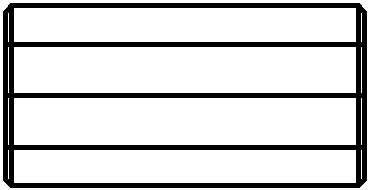
\includegraphics[scale=0.5]{taotongfront.png}}\hspace{15pt}
\subfloat[左视图]{\label{fig:taotongleft}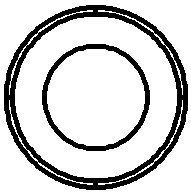
\includegraphics[scale=0.5]{taotongleft.png}}\hspace{15pt}
\subfloat[俯视图]{\label{fig:taotongtop}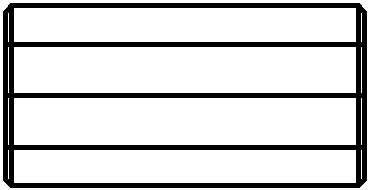
\includegraphics[scale=0.5]{taotongfront.png}}
\end{figure}
\end{procedure}

从上面的简单检验结果来看,我们套筒零件的三维建模是正确。其实,这种简单的检验方法将在AutoCAD的建模过程中会经常用到,尽管他与实际工作图存在一定的差别,但是它的操作步骤简便,能够快速地验证结果,能够有效地辅助三维建模,比较实用。
\endinput
\section{小结}
本章通过套筒零件的三维模型的构建,介绍了利用AutoCAD的圆柱体命令构建套筒的外形实体和内孔实全,并利用并集命令实现孔洞的构建,最后运用倒角边命令来实现三维倒角,整个过程化繁为简。化繁为简一种重要的思维方法。另一个方面,我们还介绍了与套筒三维模型构建的三视图知识,掌握必要的视图知识,是准确构建三维模型的基础,需要在练习中逐步掌握和运用三视图的支应规律,分析零件的重要组成部分。
\endinput
\endinput